\documentclass[aspectratio=169,10pt]{beamer}
\usepackage[T1]{fontenc}
\usepackage{lmodern}
\usepackage{amsmath,amssymb}
\usepackage{tikz}
\usetikzlibrary{arrows.meta,calc,decorations.pathmorphing,positioning}

\definecolor{ink}{HTML}{202124}
\definecolor{inkgray}{HTML}{6B7280}
\definecolor{paper}{HTML}{FFFFFF}
\definecolor{labelbg}{HTML}{F3F4F6}
\definecolor{accentgreen}{HTML}{16803C}
\definecolor{accentred}{HTML}{C62828}
\definecolor{accentblue}{HTML}{2563EB}
\definecolor{accentorange}{HTML}{B45309}
\definecolor{grnbg}{HTML}{EAF7EE}
\definecolor{redbg}{HTML}{FDEAEA}
\definecolor{blubg}{HTML}{EAF1FF}
\definecolor{orangebg}{HTML}{FFF4E5}

\setbeamertemplate{navigation symbols}{}
\setbeamercolor{normal text}{fg=ink,bg=white}
\setbeamercolor{frametitle}{fg=ink}
\setbeamerfont{frametitle}{series=\bfseries,size=\Large}
\setbeamertemplate{frametitle}{\vspace{0.16cm}\insertframetitle\par\vspace{0.05cm}\hrule height 0.4pt\vspace{0.18cm}}

\newcommand{\jj}{\mathrm{j}}
\newcommand{\rx}{\mathrm{rx}}
\newcommand{\tx}{\mathrm{tx}}
\newcommand{\smallnote}[1]{\begin{center}{\scriptsize\itshape\color{inkgray}#1}\end{center}}

\tikzset{
  flowarr/.style={-{Latex[length=2.2mm,width=1.6mm]},line width=0.75pt},
  softarr/.style={-{Latex[length=1.8mm,width=1.2mm]},line width=0.55pt,color=inkgray},
  greencard/.style={draw=accentgreen,fill=grnbg,line width=0.8pt,rounded corners=2pt,align=center,inner sep=5pt,font=\small},
  redcard/.style={draw=accentred,fill=redbg,line width=0.8pt,rounded corners=2pt,align=center,inner sep=5pt,font=\small},
  bluecard/.style={draw=accentblue,fill=blubg,line width=0.8pt,rounded corners=2pt,align=center,inner sep=5pt,font=\small},
  orangecard/.style={draw=accentorange,fill=orangebg,line width=0.8pt,rounded corners=2pt,align=center,inner sep=5pt,font=\small},
  notecard/.style={draw=ink,fill=paper,line width=0.55pt,rounded corners=2pt,align=center,inner sep=5pt,font=\small},
  tinybox/.style={draw=inkgray,fill=paper,line width=0.4pt,rounded corners=1pt,align=center,inner sep=3pt,font=\scriptsize}
}

\begin{document}

% =====================================================================
\begin{frame}[plain]
\centering
\vspace{0.75cm}
{\bfseries\Huge ICI is an unfinished loop\par}
\vspace{0.22cm}
{\Large From modulation to demodulation in OFDM\par}
\vspace{0.65cm}
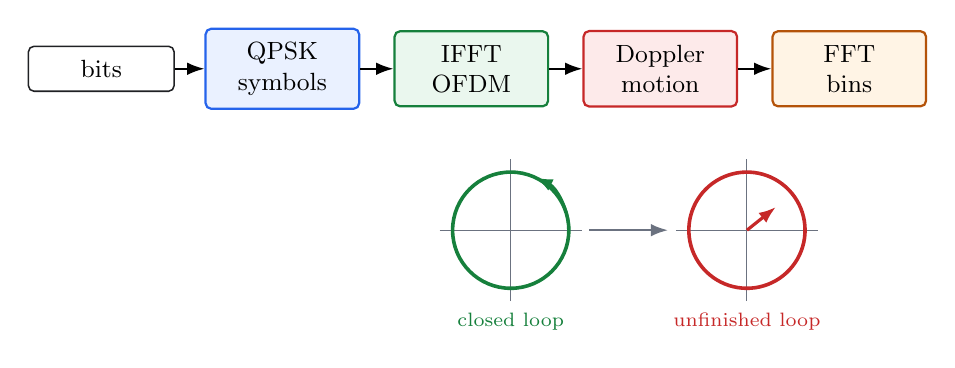
\begin{tikzpicture}[x=1cm,y=1cm,>=Latex]
  \node[notecard,minimum width=1.85cm] (bits) at (-5.2,0) {bits};
  \node[bluecard,minimum width=1.95cm] (mod) at (-2.9,0) {QPSK\\symbols};
  \node[greencard,minimum width=1.95cm] (ifft) at (-0.5,0) {IFFT\\OFDM};
  \node[redcard,minimum width=1.95cm] (dop) at (1.9,0) {Doppler\\motion};
  \node[orangecard,minimum width=1.95cm] (fft) at (4.3,0) {FFT\\bins};
  \draw[flowarr] (bits) -- (mod);
  \draw[flowarr] (mod) -- (ifft);
  \draw[flowarr] (ifft) -- (dop);
  \draw[flowarr] (dop) -- (fft);

  \begin{scope}[shift={(0,-2.05)},scale=0.82]
    \draw[inkgray] (-1.1,0)--(1.1,0);
    \draw[inkgray] (0,-1.1)--(0,1.1);
    \draw[accentgreen,line width=1.3pt] (0,0) circle (0.90);
    \draw[flowarr,color=accentgreen,line width=1.0pt] (0.90,0) arc (0:65:0.90);
    \node[font=\scriptsize\color{accentgreen}] at (0,-1.42) {closed loop};
  \end{scope}
  \draw[flowarr,color=inkgray,line width=0.9pt] (1.0,-2.05) -- (2.0,-2.05);
  \begin{scope}[shift={(3.0,-2.05)},scale=0.82]
    \draw[inkgray] (-1.1,0)--(1.1,0);
    \draw[inkgray] (0,-1.1)--(0,1.1);
    \draw[accentred,line width=1.3pt,domain=0:430,samples=100]
      plot ({0.90*cos(\x)},{0.90*sin(\x)});
    \draw[flowarr,color=accentred,line width=1.15pt] (0,0)--(0.45,0.36);
    \node[font=\scriptsize\color{accentred}] at (0,-1.42) {unfinished loop};
  \end{scope}
\end{tikzpicture}
\vspace{0.25cm}
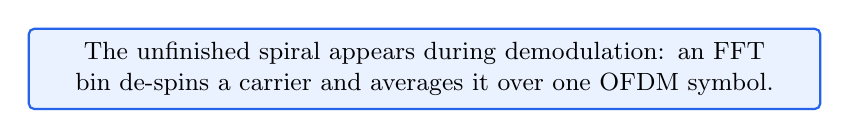
\begin{tikzpicture}
\node[bluecard,text width=0.80\linewidth]{The unfinished spiral appears during demodulation: an FFT bin de-spins a carrier and averages it over one OFDM symbol.};
\end{tikzpicture}
\end{frame}

% =====================================================================
\begin{frame}{The full OFDM chain in one picture}
\small
\begin{center}
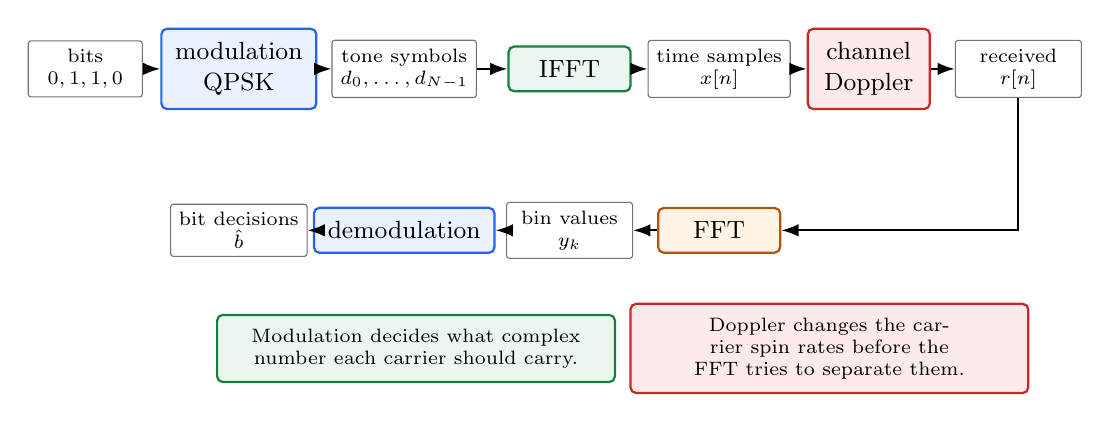
\begin{tikzpicture}[x=1cm,y=1cm,>=Latex]
  \node[tinybox,minimum width=1.45cm] (b) at (-5.6,0.8) {bits\\$0,1,1,0$};
  \node[bluecard,minimum width=1.65cm] (m) at (-3.65,0.8) {modulation\\QPSK};
  \node[tinybox,minimum width=1.75cm] (d) at (-1.55,0.8) {tone symbols\\$d_0,\ldots,d_{N-1}$};
  \node[greencard,minimum width=1.55cm] (i) at (0.55,0.8) {IFFT};
  \node[tinybox,minimum width=1.60cm] (x) at (2.45,0.8) {time samples\\$x[n]$};
  \node[redcard,minimum width=1.55cm] (ch) at (4.35,0.8) {channel\\Doppler};
  \node[tinybox,minimum width=1.60cm] (r) at (6.25,0.8) {received\\$r[n]$};

  \node[orangecard,minimum width=1.55cm] (f) at (2.45,-1.25) {FFT};
  \node[tinybox,minimum width=1.60cm] (y) at (0.55,-1.25) {bin values\\$y_k$};
  \node[bluecard,minimum width=1.65cm] (dem) at (-1.55,-1.25) {demodulation};
  \node[tinybox,minimum width=1.45cm] (bh) at (-3.65,-1.25) {bit decisions\\$\hat b$};

  \draw[flowarr] (b) -- (m); \draw[flowarr] (m) -- (d); \draw[flowarr] (d) -- (i);
  \draw[flowarr] (i) -- (x); \draw[flowarr] (x) -- (ch); \draw[flowarr] (ch) -- (r);
  \draw[flowarr] (r.south) |- (f.east); \draw[flowarr] (f) -- (y); \draw[flowarr] (y) -- (dem); \draw[flowarr] (dem) -- (bh);

  \node[greencard,text width=4.7cm,font=\scriptsize] at (-1.4,-2.75)
    {Modulation decides what complex number each carrier should carry.};
  \node[redcard,text width=4.7cm,font=\scriptsize] at (3.85,-2.75)
    {Doppler changes the carrier spin rates before the FFT tries to separate them.};
\end{tikzpicture}
\end{center}
\smallnote{The loop picture lives inside the FFT block: FFT demodulation is de-spinning plus averaging.}
\end{frame}

% =====================================================================
\begin{frame}{1. Modulation: bits become tone symbols}
\small
\begin{columns}[T,onlytextwidth]
\begin{column}{0.48\textwidth}
A modulator maps groups of bits to complex constellation points. For QPSK:
\[
  00\mapsto 1+\jj,\quad
  01\mapsto 1-\jj,\quad
  10\mapsto -1+\jj,\quad
  11\mapsto -1-\jj .
\]
Then OFDM places these complex numbers into frequency bins:
\[
  \mathbf d=[d_0,d_1,\ldots,d_{N-1}].
\]

\begin{tikzpicture}
\node[bluecard,text width=0.92\linewidth,font=\scriptsize]{A tone symbol $d_\ell$ is not yet a time waveform. It is the complex weight placed on carrier $\ell$.};
\end{tikzpicture}
\end{column}
\begin{column}{0.50\textwidth}
\begin{center}
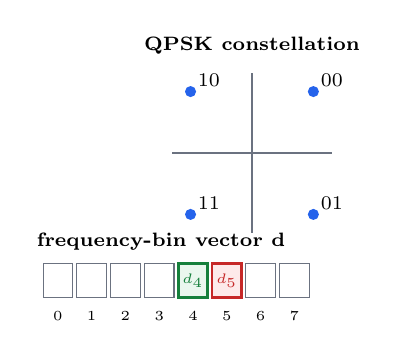
\begin{tikzpicture}[x=0.78cm,y=0.78cm,>=Latex]
  \draw[inkgray] (-1.3,0)--(1.3,0);
  \draw[inkgray] (0,-1.3)--(0,1.3);
  \foreach \x/\y/\lab in {1/1/$00$,1/-1/$01$,-1/1/$10$,-1/-1/$11$} {
    \fill[accentblue] (\x,\y) circle (2pt);
    \node[font=\scriptsize] at (\x+0.30,\y+0.18) {\lab};
  }
  \node[font=\scriptsize\bfseries] at (0,1.75) {QPSK constellation};

  \foreach \i in {0,...,7} {
    \draw[draw=inkgray,fill=paper,line width=0.4pt] ({-3.4+0.55*\i},-2.35) rectangle ++(0.48,0.55);
    \node[font=\tiny] at ({-3.16+0.55*\i},-2.65) {\i};
  }
  \draw[draw=accentgreen,line width=1.0pt,fill=grnbg] ({-3.4+0.55*4},-2.35) rectangle ++(0.48,0.55);
  \draw[draw=accentred,line width=1.0pt,fill=redbg] ({-3.4+0.55*5},-2.35) rectangle ++(0.48,0.55);
  \node[font=\tiny\color{accentgreen}] at ({-3.16+0.55*4},-2.08) {$d_4$};
  \node[font=\tiny\color{accentred}] at ({-3.16+0.55*5},-2.08) {$d_5$};
  \node[font=\scriptsize\bfseries] at (-1.48,-1.45) {frequency-bin vector $\mathbf d$};
\end{tikzpicture}
\end{center}
\end{column}
\end{columns}
\end{frame}

% =====================================================================
\begin{frame}{2. OFDM modulation: the IFFT makes spinning carriers}
\small
\begin{columns}[T,onlytextwidth]
\begin{column}{0.52\textwidth}
The IFFT converts tone symbols into time samples:
\[
  x[n]=\frac{1}{N}\sum_{\ell=0}^{N-1} d_\ell e^{\jj 2\pi \ell n/N}.
\]
This means carrier $\ell$ contributes
\[
  d_\ell e^{\jj 2\pi \ell n/N}.
\]
So carrier $\ell$ is a clock that makes exactly $\ell$ turns over one OFDM symbol.
\vspace{0.12cm}

\begin{tikzpicture}
\node[greencard,text width=0.92\linewidth,font=\scriptsize]{The transmitter deliberately chooses integer-turn clocks. That is what makes clean FFT demodulation possible.};
\end{tikzpicture}
\end{column}
\begin{column}{0.46\textwidth}
\begin{center}
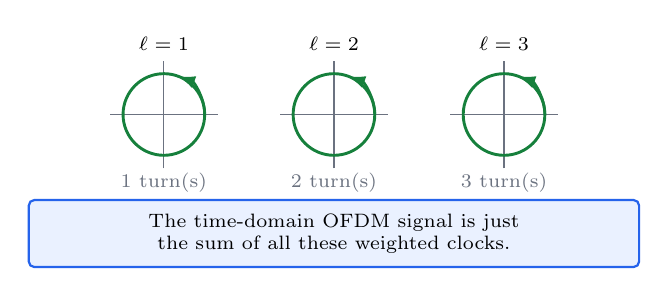
\begin{tikzpicture}[x=0.72cm,y=0.72cm,>=Latex]
  \foreach \k/\dx in {1/-3.0,2/0,3/3.0} {
    \begin{scope}[shift={(\dx,0)}]
      \draw[inkgray] (-0.95,0)--(0.95,0);
      \draw[inkgray] (0,-0.95)--(0,0.95);
      \draw[accentgreen,line width=1.05pt] (0,0) circle (0.72);
      \draw[flowarr,color=accentgreen,line width=0.95pt] (0.72,0) arc (0:70:0.72);
      \node[font=\scriptsize\bfseries] at (0,1.25) {$\ell=\k$};
      \node[font=\scriptsize\color{inkgray}] at (0,-1.20) {\k\ turn(s)};
    \end{scope}
  }
  \node[bluecard,text width=7.4cm,font=\scriptsize] at (0,-2.1)
    {The time-domain OFDM signal is just the sum of all these weighted clocks.};
\end{tikzpicture}
\end{center}
\end{column}
\end{columns}
\end{frame}

% =====================================================================
\begin{frame}{3. Demodulation: each FFT bin de-spins and averages}
\small
\begin{columns}[T,onlytextwidth]
\begin{column}{0.52\textwidth}
FFT bin $k$ asks:
\begin{center}
\emph{``How much of carrier $k$ is inside the received signal?''}
\end{center}
It does this in two steps:
\[
  \text{de-spin by } e^{-\jj 2\pi k n/N},
  \qquad
  \text{then average over } n.
\]
For one incoming carrier $\ell$, bin $k$ sees
\[
  e^{\jj 2\pi \ell n/N}\,e^{-\jj 2\pi k n/N}
  =e^{\jj 2\pi(\ell-k)n/N}.
\]
This leftover rotation is the loop we draw.
\end{column}
\begin{column}{0.46\textwidth}
\begin{center}
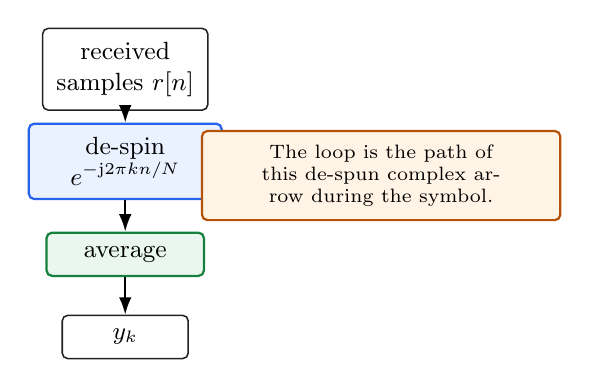
\begin{tikzpicture}[x=1cm,y=1cm,>=Latex]
  \node[notecard,minimum width=2.0cm] (r) at (0,1.35) {received\\samples $r[n]$};
  \node[bluecard,minimum width=2.45cm] (d) at (0,0.18) {de-spin\\$e^{-\jj2\pi k n/N}$};
  \node[greencard,minimum width=2.0cm] (a) at (0,-1.00) {average};
  \node[notecard,minimum width=1.6cm] (yk) at (0,-2.05) {$y_k$};
  \draw[flowarr] (r) -- (d); \draw[flowarr] (d) -- (a); \draw[flowarr] (a) -- (yk);

  \node[orangecard,text width=4.2cm,font=\scriptsize] at (3.25,0.0)
    {The loop is the path of this de-spun complex arrow during the symbol.};
\end{tikzpicture}
\end{center}
\end{column}
\end{columns}
\end{frame}

% =====================================================================
\begin{frame}{4. Clean OFDM: unwanted carriers close their loops}
\small
\begin{columns}[T,onlytextwidth]
\begin{column}{0.48\textwidth}
For a neighbouring carrier $\ell\neq k$, the leftover turn count is
\[
  \Delta_{k,\ell}=\ell-k.
\]
This is an integer. Therefore the de-spun arrow completes a whole number of loops:
\[
  c_{k,\ell}^{(0)}
  =\frac{1}{N}\sum_{n=0}^{N-1}
  e^{\jj2\pi(\ell-k)n/N}=0.
\]
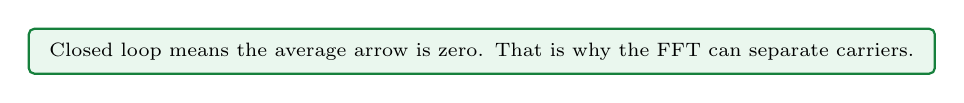
\begin{tikzpicture}
\node[greencard,text width=0.92\linewidth,font=\scriptsize]{Closed loop means the average arrow is zero. That is why the FFT can separate carriers.};
\end{tikzpicture}
\end{column}
\begin{column}{0.50\textwidth}
\begin{center}
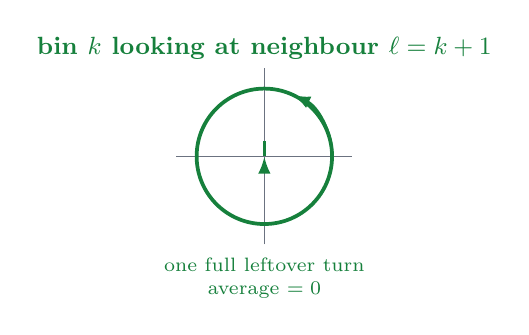
\begin{tikzpicture}[x=0.86cm,y=0.86cm,>=Latex]
  \node[font=\small\bfseries\color{accentgreen}] at (0,2.05) {bin $k$ looking at neighbour $\ell=k+1$};
  \draw[inkgray] (-1.3,0.45)--(1.3,0.45);
  \draw[inkgray] (0,-0.85)--(0,1.75);
  \draw[accentgreen,line width=1.35pt] (0,0.45) circle (1.0);
  \draw[flowarr,color=accentgreen,line width=1.0pt] (1.0,0.45) arc (0:65:1.0);
  \draw[flowarr,color=accentgreen,line width=1.1pt] (0,0.45)--(0.0,0.45);
  \node[font=\scriptsize\color{accentgreen},align=center] at (0,-1.35)
    {one full leftover turn\\average $=0$};
\end{tikzpicture}
\end{center}
\end{column}
\end{columns}
\end{frame}

% =====================================================================
\begin{frame}{5. Where the unfinished spiral comes from}
\small
\begin{columns}[T,onlytextwidth]
\begin{column}{0.52\textwidth}
Doppler slightly changes the frequency of each arriving carrier. A simple wideband model is
\[
  f_\ell^{\rx}=(1+a)\ell+\nu,
\]
where $a$ is Doppler scaling and $\nu$ is a common frequency offset.

After FFT bin $k$ de-spins by its own carrier, the leftover turn count becomes
\[
  \Delta_{k,\ell}=f_\ell^{\rx}-k
  = (\ell-k)+a\ell+\nu.
\]
The first part, $\ell-k$, is an integer. The Doppler part, $a\ell+\nu$, is usually fractional.
\vspace{0.1cm}
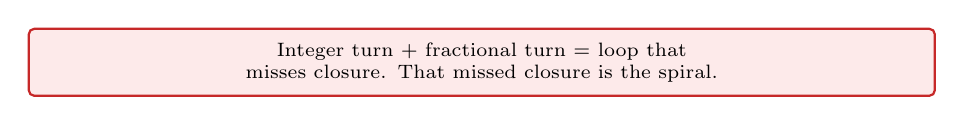
\begin{tikzpicture}
\node[redcard,text width=0.92\linewidth,font=\scriptsize]{Integer turn $+$ fractional turn $=$ loop that misses closure. That missed closure is the spiral.};
\end{tikzpicture}
\end{column}
\begin{column}{0.46\textwidth}
\begin{center}
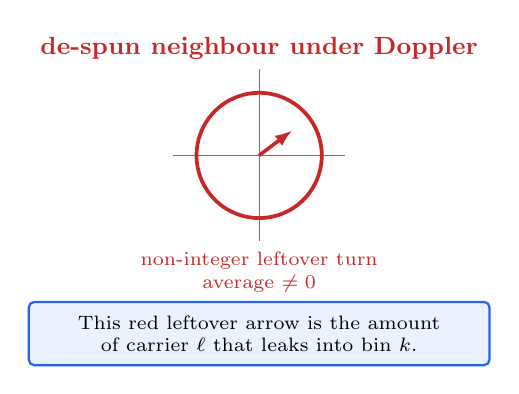
\begin{tikzpicture}[x=0.78cm,y=0.78cm,>=Latex]
  \node[font=\small\bfseries\color{accentred}] at (0,2.30) {de-spun neighbour under Doppler};
  \draw[inkgray] (-1.4,0.55)--(1.4,0.55);
  \draw[inkgray] (0,-0.85)--(0,1.95);
  \draw[accentred,line width=1.35pt,domain=0:430,samples=100]
    plot ({1.02*cos(\x)},{0.55+1.02*sin(\x)});
  \draw[flowarr,color=accentred,line width=1.3pt] (0,0.55)--(0.54,0.96);
  \node[font=\scriptsize\color{accentred},align=center] at (0,-1.35)
    {non-integer leftover turn\\average $\neq 0$};
  \node[bluecard,text width=5.5cm,font=\scriptsize] at (0,-2.35)
    {This red leftover arrow is the amount of carrier $\ell$ that leaks into bin $k$.};
\end{tikzpicture}
\end{center}
\end{column}
\end{columns}
\end{frame}

% =====================================================================
\begin{frame}{6. The leftover average is the ICI coefficient}
\small
\begin{columns}[T,onlytextwidth]
\begin{column}{0.52\textwidth}
For one carrier $\ell$ entering FFT bin $k$, define
\[
  c_{k,\ell}
  =\int_0^1 e^{\jj2\pi\Delta_{k,\ell}t}\,dt.
\]
This is the average of the de-spun rotating arrow.

Clean OFDM:
\[
  \Delta_{k,\ell}=\ell-k \quad\Rightarrow\quad c_{k,\ell}=0,
  \qquad \ell\neq k.
\]
Doppler OFDM:
\[
  \Delta_{k,\ell}=(\ell-k)+a\ell+\nu
  \quad\Rightarrow\quad c_{k,\ell}\neq 0.
\]
\end{column}
\begin{column}{0.46\textwidth}
\begin{center}
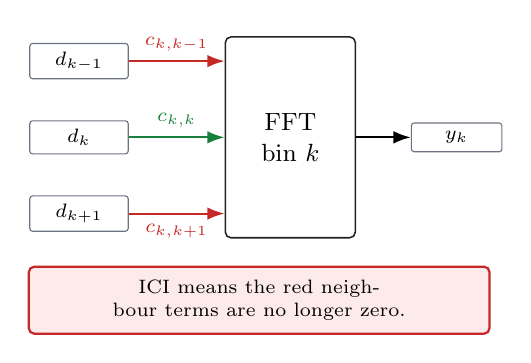
\begin{tikzpicture}[x=0.88cm,y=0.88cm,>=Latex]
  \node[tinybox,minimum width=1.25cm] (d3) at (-2.4,1.2) {$d_{k-1}$};
  \node[tinybox,minimum width=1.25cm] (d4) at (-2.4,0.1) {$d_k$};
  \node[tinybox,minimum width=1.25cm] (d5) at (-2.4,-1.0) {$d_{k+1}$};
  \node[notecard,minimum width=1.65cm,minimum height=2.55cm] (bin) at (0.65,0.1) {FFT\\bin $k$};
  \node[tinybox,minimum width=1.15cm] (y) at (3.05,0.1) {$y_k$};
  \draw[flowarr,color=accentred] (d3) -- node[above,font=\scriptsize] {$c_{k,k-1}$} (bin.west |- d3);
  \draw[flowarr,color=accentgreen] (d4) -- node[above,font=\scriptsize] {$c_{k,k}$} (bin.west);
  \draw[flowarr,color=accentred] (d5) -- node[below,font=\scriptsize] {$c_{k,k+1}$} (bin.west |- d5);
  \draw[flowarr] (bin) -- (y);
  \node[redcard,text width=5.5cm,font=\scriptsize] at (0.2,-2.25)
    {ICI means the red neighbour terms are no longer zero.};
\end{tikzpicture}
\end{center}
\end{column}
\end{columns}
\end{frame}

% =====================================================================
\begin{frame}{7. Demodulation now sees a sum, not a single symbol}
\small
\begin{columns}[T,onlytextwidth]
\begin{column}{0.49\textwidth}
Clean OFDM gives one bin, one symbol:
\[
  y_k=c_{k,k}d_k+n_k.
\]
With Doppler, the same FFT bin receives leakage from neighbours:
\[
  y_k=c_{k,k}d_k+
  \sum_{\ell\neq k} c_{k,\ell}d_\ell+n_k.
\]
The unwanted terms are inter-carrier interference:
\[
  \mathrm{ICI}_k=\sum_{\ell\neq k} c_{k,\ell}d_\ell.
\]

\begin{tikzpicture}
\node[bluecard,text width=0.92\linewidth,font=\scriptsize]{So the phrase ``ICI is an unfinished loop'' means: each nonzero off-diagonal coefficient is a failed cancellation loop.};
\end{tikzpicture}
\end{column}
\begin{column}{0.49\textwidth}
\begin{center}
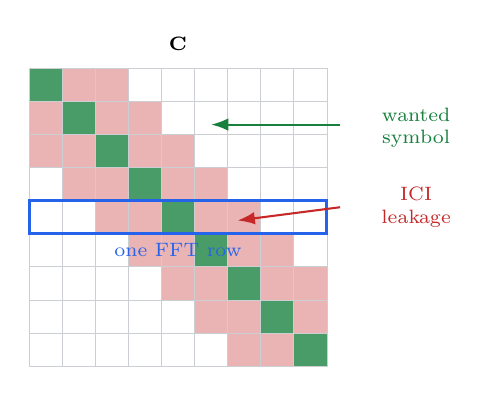
\begin{tikzpicture}[x=0.42cm,y=0.42cm]
  \foreach \r in {0,...,8} {
    \foreach \c in {0,...,8} {
      \pgfmathtruncatemacro{\dist}{abs(\r-\c)}
      \ifnum\dist=0
        \fill[accentgreen!78] (\c,8-\r) rectangle ++(1,1);
      \else
        \ifnum\dist<3
          \fill[accentred!35] (\c,8-\r) rectangle ++(1,1);
        \else
          \fill[paper] (\c,8-\r) rectangle ++(1,1);
        \fi
      \fi
      \draw[inkgray!35,line width=0.2pt] (\c,8-\r) rectangle ++(1,1);
    }
  }
  \draw[accentblue,line width=1.1pt] (0,4) rectangle (9,5);
  \node[font=\scriptsize\bfseries] at (4.5,9.75) {$\mathbf C$};
  \node[font=\scriptsize\color{accentblue}] at (4.5,3.52) {one FFT row};
  \node[font=\scriptsize\color{accentgreen},align=center] at (11.7,7.2) {wanted\\symbol};
  \node[font=\scriptsize\color{accentred},align=center] at (11.7,4.8) {ICI\\leakage};
  \draw[flowarr,color=accentgreen] (9.4,7.3)--(5.5,7.3);
  \draw[flowarr,color=accentred] (9.4,4.8)--(6.3,4.4);
\end{tikzpicture}
\end{center}
\end{column}
\end{columns}
\end{frame}

% =====================================================================
\begin{frame}{Final takeaway}
\small
\begin{center}
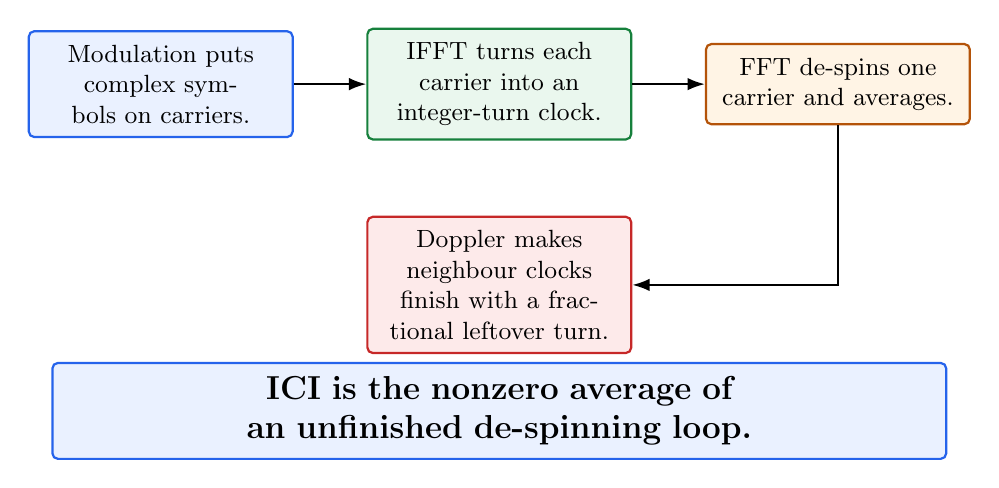
\begin{tikzpicture}[x=1cm,y=1cm,>=Latex]
  \node[bluecard,text width=3.0cm] (mod) at (-4.3,1.1) {Modulation puts complex symbols on carriers.};
  \node[greencard,text width=3.0cm] (ifft) at (0,1.1) {IFFT turns each carrier into an integer-turn clock.};
  \node[orangecard,text width=3.0cm] (fft) at (4.3,1.1) {FFT de-spins one carrier and averages.};
  \node[redcard,text width=3.0cm] (dop) at (0,-1.45) {Doppler makes neighbour clocks finish with a fractional leftover turn.};
  \draw[flowarr] (mod) -- (ifft); \draw[flowarr] (ifft) -- (fft); \draw[flowarr] (fft.south) |- (dop.east);

  \node[bluecard,text width=11.0cm,font=\large] at (0,-3.05)
    {\textbf{ICI is the nonzero average of an unfinished de-spinning loop.}};
\end{tikzpicture}
\end{center}
\end{frame}

\end{document}
